%!TEX root = ../Thesis.tex

\chapter{Untersuchung verschiedener Straßentopologien}
\label{cha:street_topologies}

% Beschreibung möglicher (Auswahl) Straßentopologien und ihrer Herausforderungen für die Erkennung von Fahrbahnen
% Idealerweise immer Bild einer entsprechenden Topologie und der entsprechenden Roh-Trajektorien
% Erläuterung: Was ist eine "Fahrspur" in dieser Arbeit. (d.h. nicht notwendigerweise eine Spur, wie sie auf Straße markiert ist.
% Beschreibt übliche Fahrbahn eines Fahrzeugs?!)

In diesem Kapitel werden häufig vorkommende Straßentopologien analysiert.
Es wird untersucht, welche Herausforderungen bei der Erkennung von Fahrspuren im Fall der unterschiedlichen
Topologien existieren.

% Landstraßen (ein / zweispurig),
\section{``Normale'' Straßenabschnitte}

Mit ``normalen'' Straßenabschnitten sind hier all jene gemeint, welche keine Kreuzung, keinen Kreisverkehr
oder ähnliches beinhalten. In einem solchen Abschnitt verlaufen Fahrspuren parallel zueinander und sind
üblicherweise klar getrennt.
Häufig zu finden sind ``normale'' Straßenabschnitte auf Landstraßen oder Autobahnen. In Abbildung
\ref{fig:topos_normal_lanes} sind zwei Beispiele normaler Straßenabschnitte dargestellt.

% TODO: 
\begin{figure}[H]
    \centering
    \subfloat[Landstraße]{{
        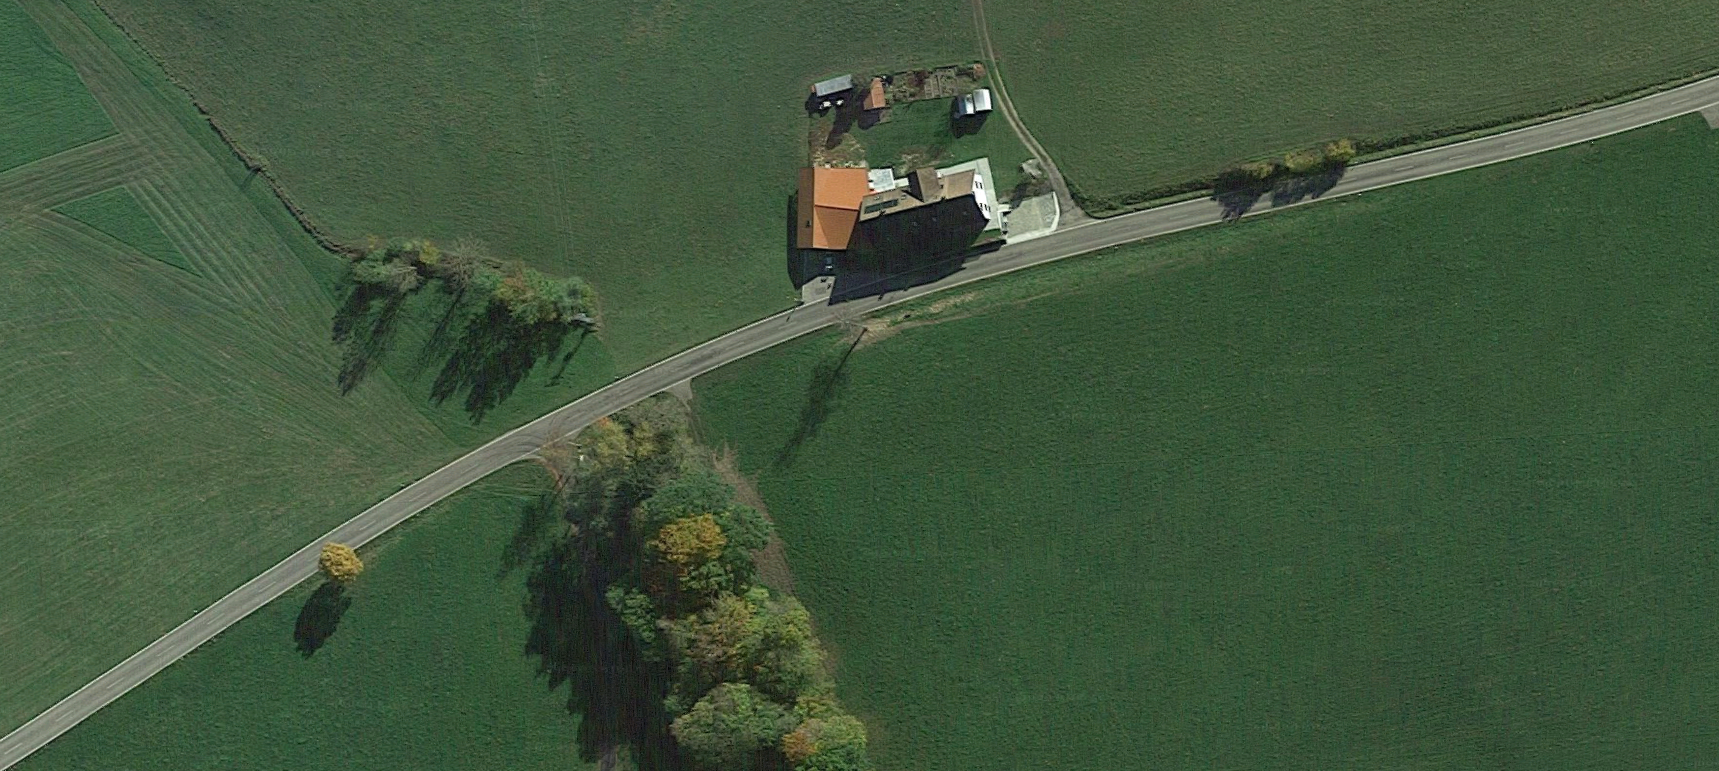
\includegraphics[align=c, width=0.40\linewidth]{resources/img/topos/landstrasse_1}
    }}
    \qquad \qquad
    \subfloat[Autobahn]{{
        \includegraphics[align=c, width=0.34\linewidth]{resources/img/topos/Autobahn}
    }}
    \caption{Beispiele normaler Straßenabschnitte}
    \label{fig:topos_normal_lanes}
\end{figure}

Unterschieden werden muss zwischen Fahrbahnen mit nur einer oder mit mehreren Fahrspuren. Besitzt
eine Fahrbahn nur eine Fahrspur und es handelt sich bei ihr nicht um eine Einbahnstraße, so bewegen
sich Fahrzeuge auf dieser Spur in beide Richtungen. Dies erschwert die Bestimmung der Fahrspuren,
da die Trajektorien der Fahrzeuge auf einer Spur in entgegengesetzte Richtungen verlaufen.
In einer solchen Situation auf Basis der Trajektorien zwei disjunkte Spuren zu identifizieren ist nicht immer möglich.
Ansonsten ist die Erkennung von Fahrspuren im Fall dieser Topologien allerdings verhältnismäßig unkompliziert,
da die Bewegungsbahnen der Fahrzeuge in der Regel gut in Cluster unterteilt werden können und keine Überlagerungen
von Spuren existieren.

% Kreuzungen (inkl. Abbiegespuren)
\section{Kreuzungen}

% Fahrbahnen kreuzen sich, geregelt über Ampelanlagen oder Rechts-vor-Links
% Abbiegespuren
% Fahrspuren überlagern sich. Sinnvolle Aufteilung

Kreuzungen stellen eine etwas kompliziertere Straßentopologie dar. Die in einem Streckenabschnitt mit
Kreuzung enthaltenen Fahrspuren verlaufen nicht alle parallel zueinander, sondern überlagern sich
Abschnittsweise. In Abbildung \ref{fig:topos_crossroad} ist beispielsweise ein Straßenabschnitt dargestellt,
in welchem sich sechs horizontal verlaufende Fahrspuren mit vier vertikal verlaufenden kreuzen.

\begin{figure}[H]
\centering
    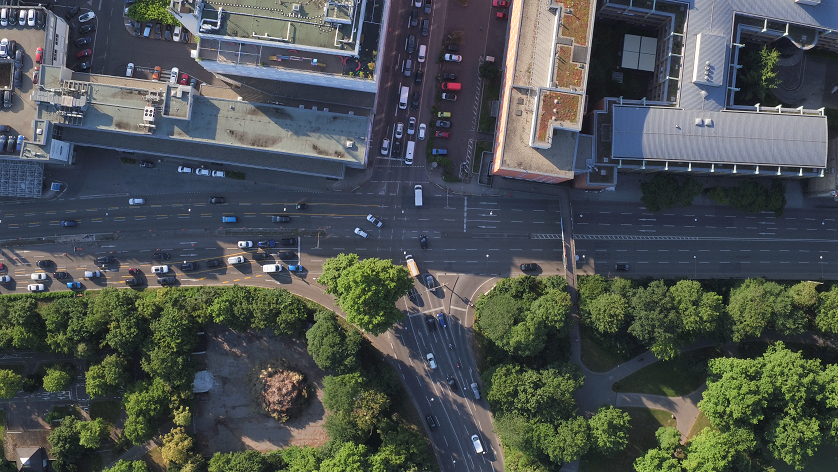
\includegraphics[width=0.5\linewidth]{resources/img/umsetzung/U1/Neckartor_Aufnahme}
\caption{Beispiel Kreuzung}
\label{fig:topos_crossroad}
\end{figure}

Es existieren mehrere Herausforderungen bei der Fahrspurerkennung auf Kreuzungen. Die größte ist, dass
aufgrund von abbiegenden Spuren sich die Trajektorien unterschiedlicher Wege durch die Kreuzung
abschnittsweise stark überlagern. Es ist wichtig, dass alle Spuren trotz Überschneidungen zuverlässig
identifiziert werden und in Bereichen, in welchen sich mehrere Spuren überlagern, alle bis auf eine
partitioniert werden. Problematisch ist zudem, dass in Kreuzungen teilweise Abbiegespuren existieren,
welche nur wenig befahren sind und über welche Fahrzeuge auf unterschiedliche andere Spuren abbiegen.
In einer Clusteranalyse werden die entsprechenden Trajektorien aufgrund ihrer unterschiedlichen Verläufe
nicht einem Cluster zugewiesen, was die Erkennung dieser Spuren erschwert.

% Kreisverkehre
\section{Kreisverkehre}

% 12 Bewegungsbahnen durch Kreisverkehr (ausgenommen 360Grad Wendungen etc.)
% schwierig zu definieren, wie fahrspuren durch Kreisverkehr verlaufen
% Welche partitionieren
% Werden alle Bahnen richtig erkannt? Viele Überdeckungen. Richtig geclusterd?

% Die Fahrspuren in Kreisverkehren besitzen grundlegend die selben

Ein Kreisverkehr ist ein alternatives Mittel zur Steuerung des Verkehrs an einem Infrastrukturknotenpunkt.
Auf seiner Kreisfahrbahn dürfen Fahrzeuge nur in Richtung gegen den Uhrzeigersinn fahren. Bei einem
Kreisverkehr mit vier Ein- und Ausfahrten ergeben sich somit 12 möglich Wege durch den Knotenpunkt,
wenn 360 Grad Wendungen ausgeklammert werden. Abbildung \ref{fig:topos_kreisel} zeigt einen typischen
Kreisverkehr.

\begin{figure}[H]
\centering
    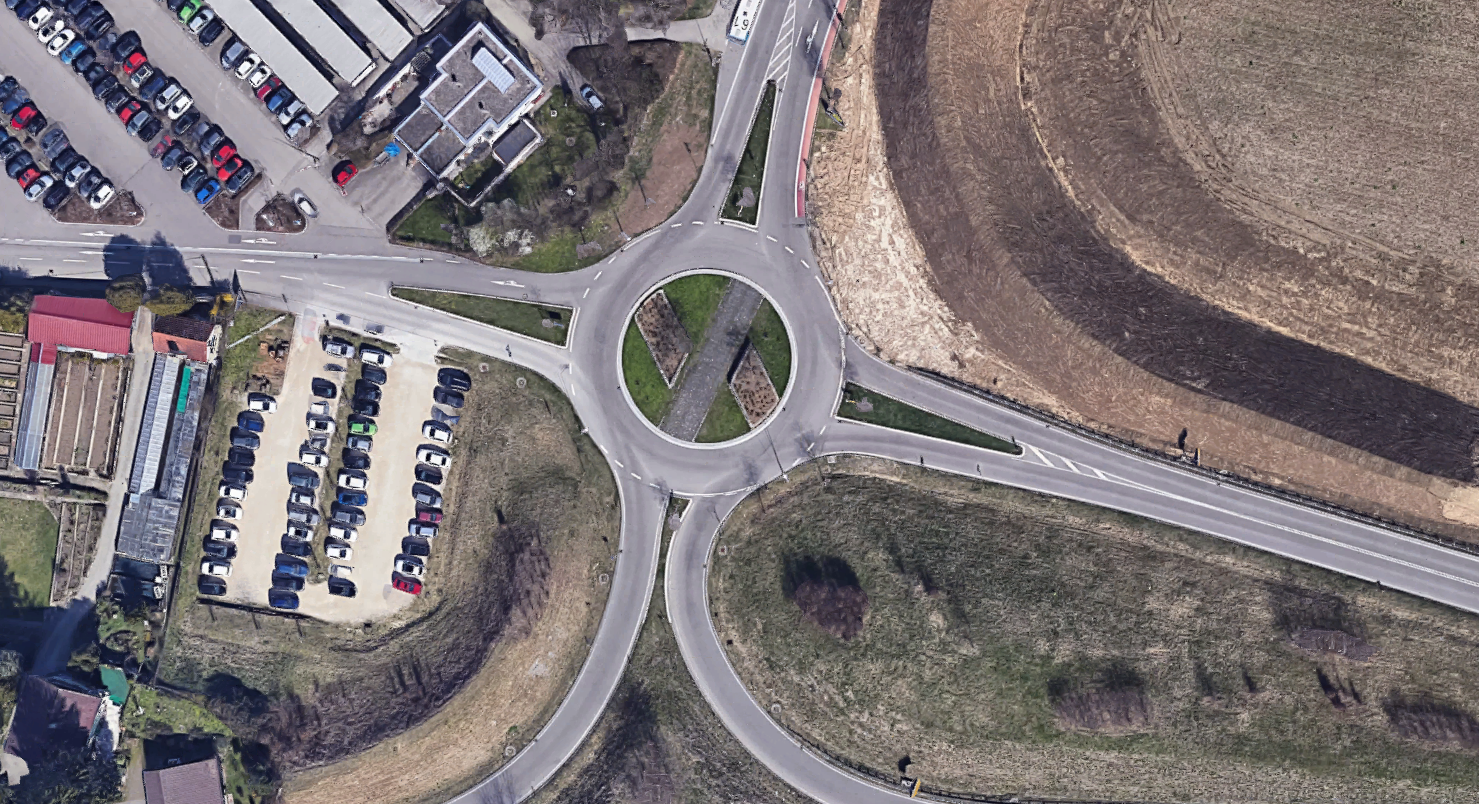
\includegraphics[width=0.5\linewidth]{resources/img/topos/kreisverkehr}
\caption{Beispiel Kreisverkehr}
\label{fig:topos_kreisel}
\end{figure}

Bei der Identifikation von Fahrspuren in Kreisverkehren besteht grundlegend die selbe Hauptschwierigkeit
wie bei der Erkennung in Kreuzungen: die einzelnen Spuren überschneiden sich. In Kreisverkehren sind
die Längen der Überschneidungen zwar geringer als in Kreuzungen, dafür existieren mehr davon.
Die Partitionierung der Fahrspuren wird komplizierter, da die Entscheidung welche Spur-Überlagerungen
zu entfernen sind, weniger eindeutig ist.

\section{Sich öffnende und schließende Fahrspuren}

Sich öffnende und schließende Fahrspuren treten in unterschiedlichen Situationen auf. In Abbildung
\ref{fig:topos_opening} ist beispielsweise ein Auf- und Abfahrt einer Autobahn dargestellt.

\begin{figure}[H]
\centering
    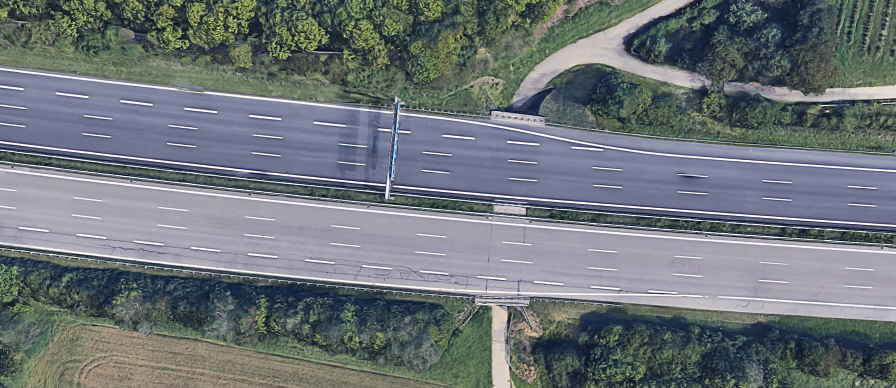
\includegraphics[width=0.5\linewidth]{resources/img/topos/opening_lane}
\caption{Beispiel Kreisverkehr}
\label{fig:topos_opening}
\end{figure}

Problematisch bei der Erkennung von sich öffnenden und schließenden Spuren ist, dass diese aus anderen
Spuren hervorgehen oder übergehen und sich in diesem Bereich verschmälern. Die auf Basis der Trajektorien
identifizierten Spuren müssen daher an der richtigen Stelle partitioniert werden und ihrer Breite
sich ihrem Verlauf entsprechend anpassen.